\section{Einleitung: Von Nullen und Einsen}
\only<article>{
  Um die Konzepte hinter aktuellen Entwicklungen wie z.B. ,,Cloud'' und BigData verstehen zu können, benötigen wir ein wenig Grundlagenwissen. Das werden wir im Laufe der Lektionen aufbauen. Mit diesem Wissen wird uns dann die Logik hinter den Entwicklungen verständlich. 

  Dazu schauen wir zunächst auf die Geschichte des Internets, befassen uns mit der Technik und bauen Verständnis für die grundlegenden Konzepte auf. 

  Wir lernen verschiedene Möglichkeiten zur Speicherung von Daten kennen, werden die unterschiedlichen Typen von Datenbanken besprechen und feststellen, dass die Tabelle nicht immer die ideale Form für das Ablegen von Daten ist, geschweige denn für die Formatierung bzw. Darstellung.

  So kommen wir dann auf Grundlagen der Formatierung von Webinhalten, die Struktur von Webseiten und die Manipulation derselben durch Javascript, gehen auf Frameworks ein und kommen schliesslich auf Webapplikationen.

  Ein Exkurs zeigt uns, wie man die bisher erlernten Konzepte und Techniken zum automatisierten Testen von Webapplikationen nutzen kann, bevor wir dann klären, was die viel gerühmte ,,Cloud'' ist und wo wir in unserer Branche beim Thema BigData stehen.
}

\only<presentation>{
\begin{frame}[label=uebersicht]{Kursus / Übersicht}
  \begin{overprint}
    \onslide<1|handout:0>
      \textbf{01.12.2017 : Von Nullen und Einsen}
      \begin{itemize}
        \item Vorstellung und Überblick
        \item Die Entwicklung des Internets
        \item Server: Was ist das eigentlich?
      \end{itemize}
    
    \onslide<2|handout:0>
      \textbf{15.12.2017 : Internettechnologien I, Datenbanktechnologien I}
      \begin{itemize}
        \item IntT I: Dokumentformen, Skriptsprachen, Ajax, responsive Web
        \item DBT I: Datenbanktypen, Technologien, Einstieg SQL
      \end{itemize}
    
    \onslide<3|handout:0>
      \textbf{22.12.2017 : Internettechnologien II: von interaktiven Webseiten zu WebApps in der Cloud}
      \begin{itemize}
        \item das ,,DOM''
        \item Manipulation von Elementen mit JavaScript
        \item Der Einsatz von JavaScript Frameworks anhand von Primos neuem UI
        \item Exkurs: Einsatz der bisher gelernten Technologien zum automatisierten Testen von WebApplikationen
      \end{itemize}
    
    \onslide<4|handout:0>
      \textbf{19.01.2018 : Datenbanktechnologien II: BigData}
      \begin{itemize}
        \item kurze Wiederholung --- wo stehen wir?
        \item Klärung verschiedener Begriffe und Buzzwords
        \item Anwendungsszenarien, Anwendung in der ETH
        \item In Medias Res: BigData am Bsp. Logfiles, DataScience am Bsp. Benutzerdaten
      \end{itemize}
  \end{overprint}
\end{frame}
}

\only<article>{
  Zunächst wollen wir uns mit der Denkweise von Informatikern vertraut machen, die für ,,normale'' Menschen etwas gewöhnungsbedürftig sein kann. 

  Informatiker lachen beispielsweise herzlich über folgenden Satz:
}

\begin{frame}{\only<presentation>{Von Nullen und Einsen}}
  \begin{quote}
    Es gibt 10 Sorten von Menschen: Diejenigen, die das Binärsystem verstehen, und die Übrigen.\hfill (Autor unbekannt)
  \end{quote}
\end{frame}

\only<article>{
  Computer basieren darauf, dass man in Schaltkreisen den Strom an-- bzw. abschalten kann. Es gibt nur die zwei Zustände ,,AN'' und ,,AUS". Mathematisch ist das kein Problem, mit jeder Anzahl von Ziffern $>2$ lässt sich zählen. Aber die Wirklichkeit lässt sich nur näherungsweise damit beschreiben.

  Der Satz macht nur dann Spass, wenn man das Binärsystem kennt und versteht. Im täglichen Leben benutzen wir das Dezimalsystem. Zum besseren Verständnis nehmen wir an, dass jeder Zahl eine unendliche Anzahl von Stellen vorangestellt ist, die den Wert 0 haben. Also statt $1$ nehmen wir $00000001$ an (hier mit sieben Stellen vorneweg, weil sich eine unendliche Anzahl so schlecht aufschreiben lässt\ldots{}).

  Wir zählen die Ziffern von $0$ bis $9$ hoch, und wenn die Ziffern aufgebraucht sind, erhöhen wir die Stelle davor um eins und setzen die eben hochgezählte Ziffer auf $0$ zurück. So wird die Zahl $9$ ($00000009$), wenn man um eins erhöht, zu $10$ ($00000010$)

  \begin{center}
    \begin{tabular}{rrrrrrcl}
      0 & 0 & 0 & 0 & 0 & 0 & 0 & 9\tabularnewline
        &  &  &  &  &  & \multicolumn{1}{c|}{+1} & auf 0 zurücksetzen\tabularnewline
      0 & 0 & 0 & 0 & 0 & 0 & 1 & 0\tabularnewline
    \end{tabular}
  \end{center}

  Im Binärsystem stehen uns nur zwei Ziffern zur Verfügung. Aber zwei Ziffern reichen zum Zählen. Man wendet das gleiche Prinzip an. So wird die Zahl $1$ ($00000001$), wenn man um eins erhöht, zu $10$ ($00000010$). Jetzt ergibt der Witz einen Sinn. Der binäre Wert $10$ entspricht in unserem Dezimalsystem dem Wert zwei.
  }

\begin{frame}{Die Folge der ersten neun Binärzahlen\ldots{}}
  \begin{center}
    0, 1, 10, 11, 100, 101, 110, 111, 1000 \ldots{}
  \end{center}
\end{frame}
%
\begin{frame}{\ldots{}und die ,,Übersetzung"}
  \begin{center}
    \begin{tabular}{|r|c|}
      \hline 
      binär & dezimal\tabularnewline
      \hline 
      \hline 
      0 & 0\tabularnewline
      \hline 
      1 & 1\tabularnewline
      \hline 
      10 & 2\tabularnewline
      \hline 
      11 & 3\tabularnewline
      \hline 
      100 & 4\tabularnewline
      \hline 
      101 & 5\tabularnewline
      \hline 
      110 & 6\tabularnewline
      \hline 
      111 & 7\tabularnewline
      \hline 
    \end{tabular}
  \end{center}
\end{frame}

\only<article>{
  Leibniz schreibt Ende des 17. Jahrhunderts dazu: 
  \begin{quotation}
    \ldots{}deshalb ist der letzte Tag der vollkommenste und der Sabbat, denn an ihm ist alles geschaffen und erfüllt, und deshalb schreibt sich die 7 111, also ohne Null. Und nur wenn man die Zahlen bloß mit 0 und 1 schreibt, erkennt man die Vollkommenheit des siebenten Tages. \hfill (Gottfried Wilhelm Leibniz)
  \end{quotation}
  Ein Computer kann aktuell\footnote{Die zur Zeit in Entwicklung befindlichen Quantencomputer kennen auch noch ,,vielleicht". Aber obwohl erste Schritte vielversprechend sind, liegen Quantencomputer noch in weiter Ferne. Und Quantenphysiker denken noch schräger als Informatiker --- das möchte ich dem geneigten Leser nicht zumuten.} nur zwei Zustände darstellen: ,,AN'' und ,,AUS". Damit ist das Binärsystem für Computer zum Rechnen ideal.

  \begin{block}{Hinweis}
    Für uns wäre es aus verschiedenen Gründen sehr unpraktisch, im Binärsystem zu rechnen. Die Zahlen werden z.B. sehr schnell sehr lang. So braucht die Sieben im Binärsystem schon drei Stellen (111).
  \end{block}

  Zahlen können wir also genau umrechnen. Aber wie bilden beispielsweise Musik digital ab? 

  Man kann sich mit ,,AN'' / ,,AUS'' -- Zuständen einer Kurve annähern. Zunächst vereinfachen wir das Problem, indem wir statt Musik eine Sinuskurve zur Veranschaulichung benutzen. Das geht, weil ein Ton eine Summe von Schwingungen ist. Sinustöne sind sehr reine Töne, deren Schwingung sehr sauber der Sinuskurve entspricht.
  }
\begin{frame}{eine Sinuskurve}
  \begin{figure}
    \begin{center}  
      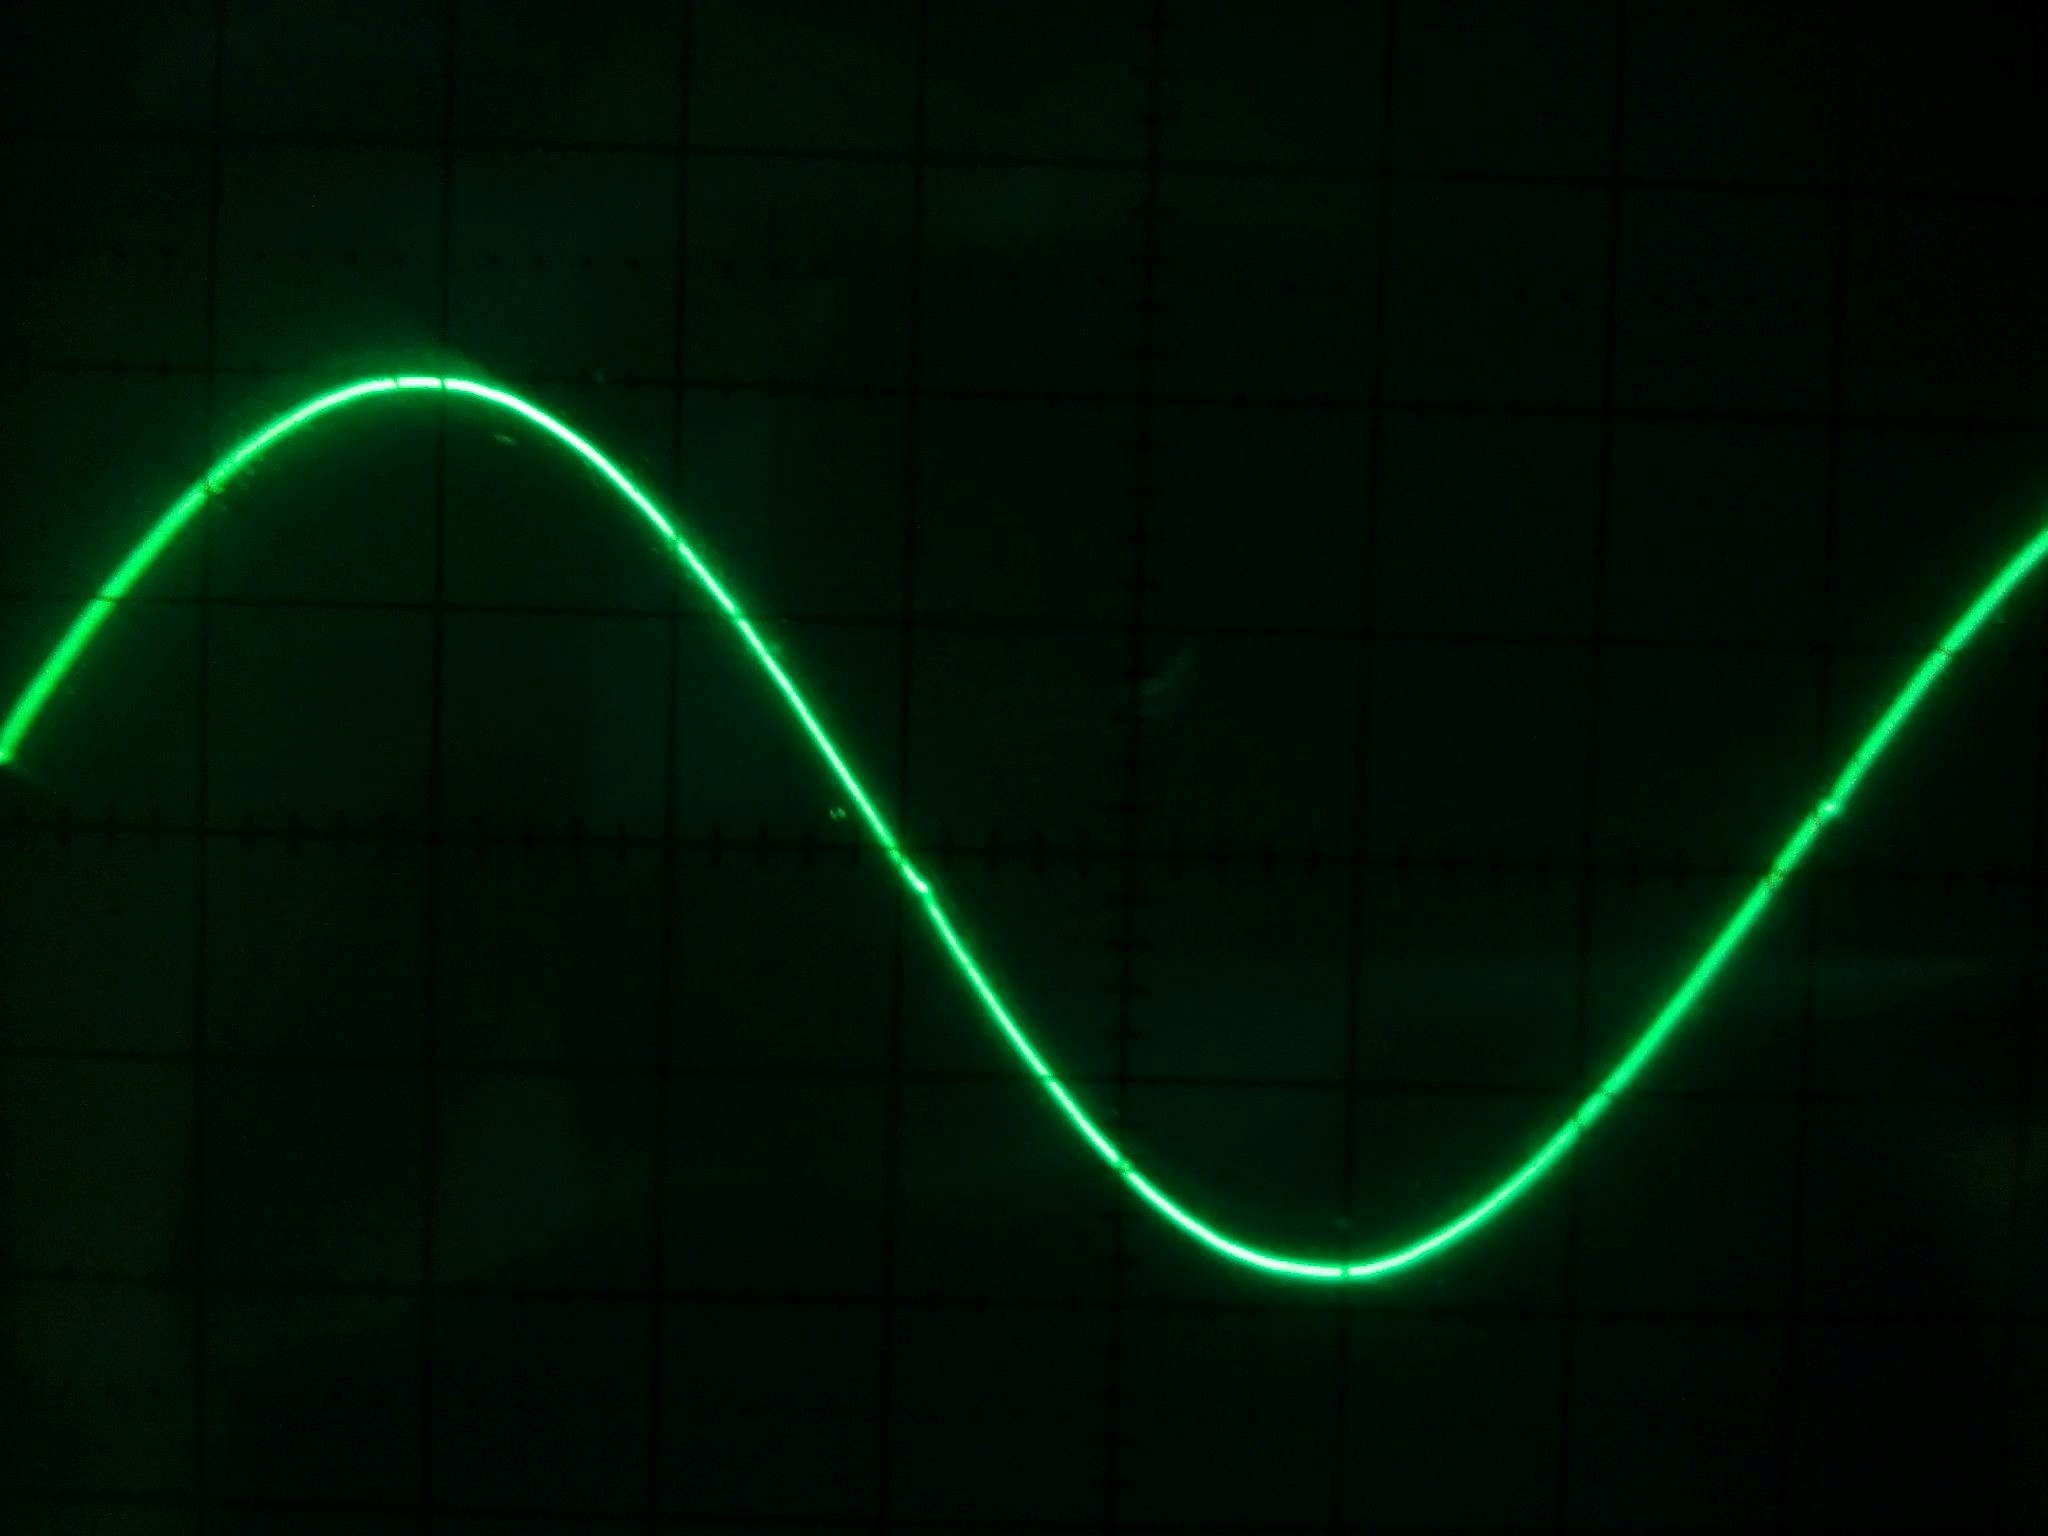
\includegraphics[width=0.8\textwidth]{pics/sinus-kurve}
    \end{center}
    \caption{Sinuskurve, Quelle: $\text{Computer:club}^2$, Urheber: Rolf Degen}
  \end{figure}
\end{frame}

\only<article>{
  Wir wollen mal versuchen, mit unseren zwei Zuständen eine solche Kurve zu erzeugen, indem wir sie auf Karos abbilden. Nehmen wir an, dass ein Karo dem Zustand ,,AN'' entspricht, kein Karo dem Zustand ,,AUS". Wenn man jetzt Karos zu einer Pyramide zusammenstellt und dahinter an der Basis genau so eine Pyramide nach unten zeigen lässt, erhält man eine Annäherung an eine Sinuskurve. Die Abbildung der Kurve sähe dann etwa aus wie folgt.
  }

\begin{frame}{eine grobe Annäherung}
  \begin{center}
    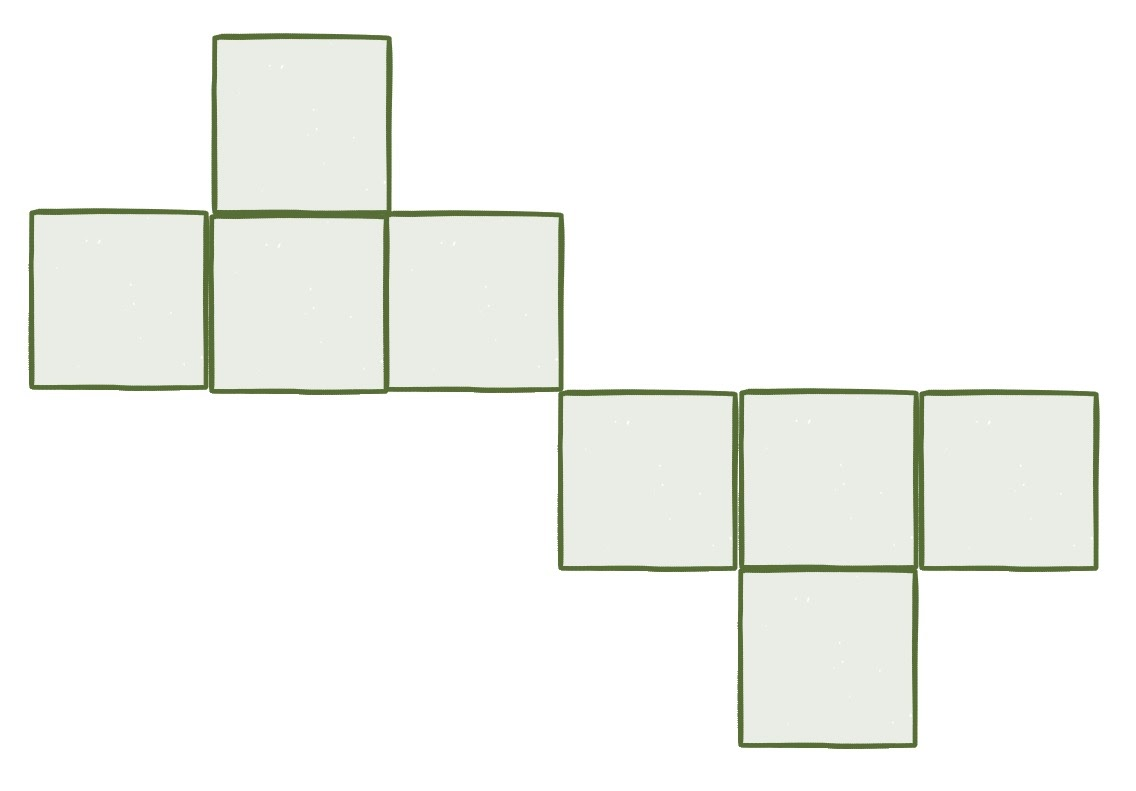
\includegraphics[width=0.8\textwidth]{pics/grobe-karos}
  \end{center}
\end{frame}

\only<article>{
  Je mehr Informationen bzw. ,,AN'' / ,,AUS'' -- Zustände wir nun verwenden, desto feiner wird die Annäherung an die Kurve:
  }

\begin{frame}{eine feinere Annäherung}
  \begin{center}
    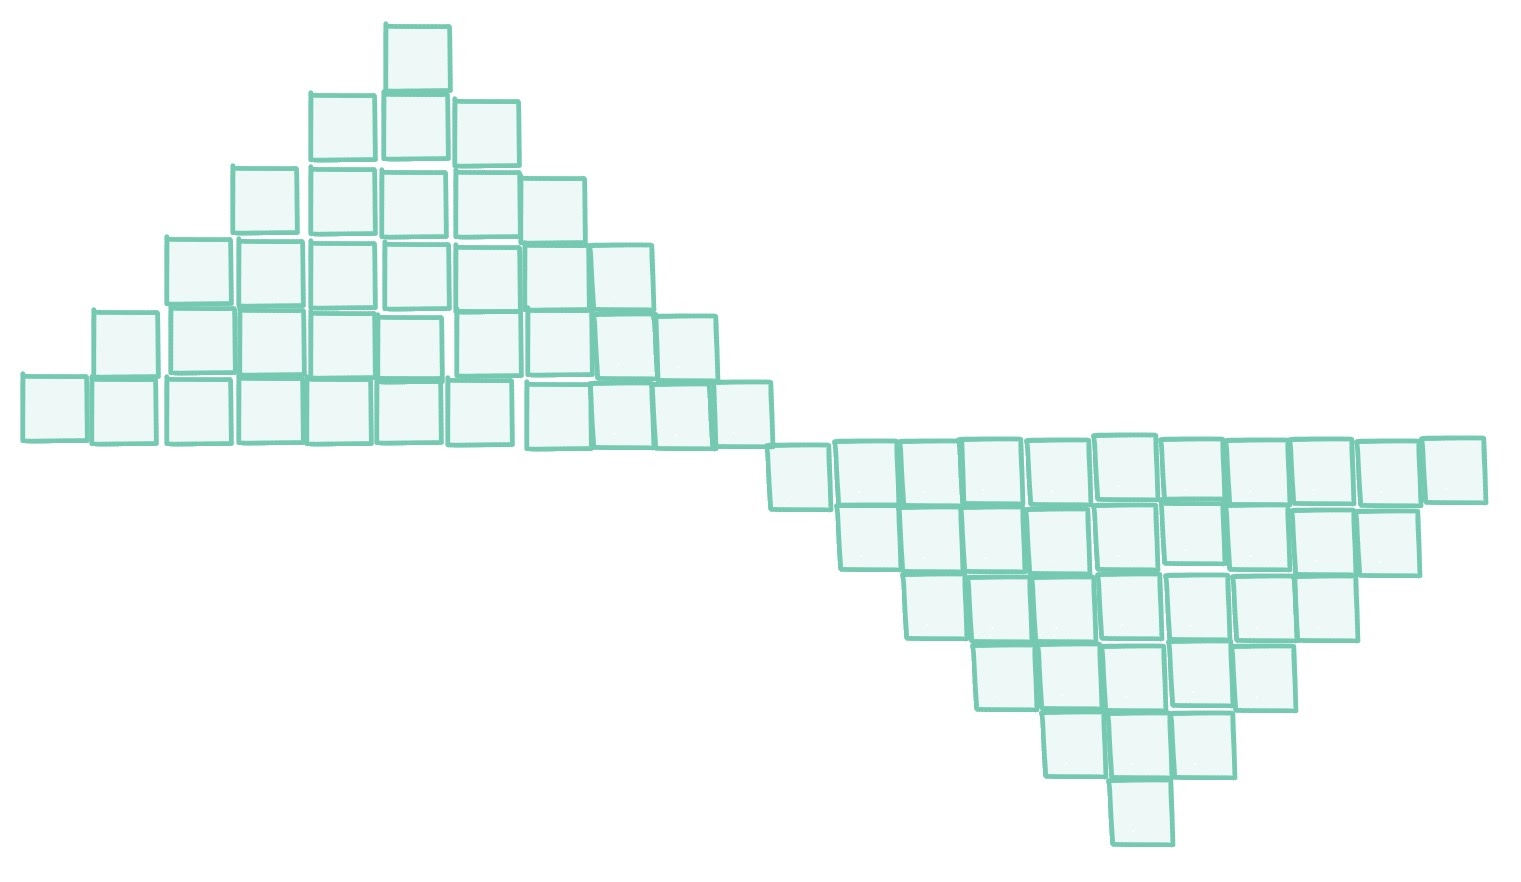
\includegraphics[width=0.8\textwidth]{pics/feine-karos}
  \end{center}
\end{frame}

\only<article>{
  Wenn man mal von meinen mangelnden Zeichenkünsten absieht, kommt das Ganze der Kurve schon näher. Da unser Auge wie unser Ohr ein begrenzt feines Messinstrument ist, brauchen wir das Karo-- Muster nur klein genug zu machen (oder weit genug vom Augen zu entfernen) und können die Treppenstufen der Karos nicht mehr sehen bzw. das Unnatürliche im Ton nicht mehr hören.

  Mit ,,AN'' / ,,AUS'' -- Zuständen lässt sich also die Wirklichkeit näherungsweise beschreiben. 
  \begin{block}{Hinweis}
  Egal, wie leistungsfähig Computersysteme sind, oder noch sein werden, sie werden immer nur eine Annäherung bieten können.
  \end{block}
  Glücklicherweise ist unser Ohr als Messinstrument so unsensibel, dass wir die Näherungen nicht mehr vom Original unterscheiden können, solange sie nur fein genug sind. So konnte Ende der siebziger Jahre die Firma Philipps der digitalen Musikproduktion und --wiedergabe mit der Einführung des CD--Spielers kräftigen Schwung geben.

  Mit Bildern ist das Prinzip ähnlich: Je feiner die Treppen, je höher also die Informationsdichte, desto wirklichkeitsgetreuer wird das Bild wiedergegeben.
  }

\begin{frame}{}
  \begin{figure}
    \begin{center}  
      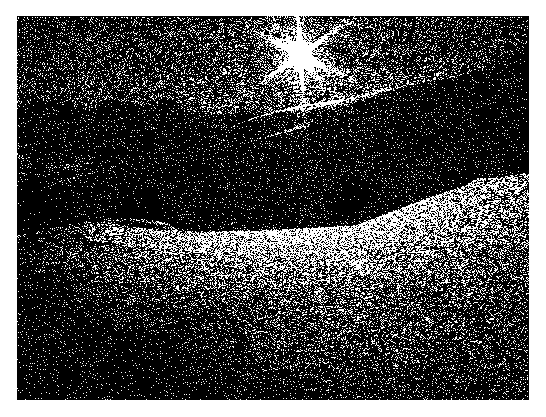
\includegraphics[width=0.8\textwidth]{pics/sw}
    \end{center}
    \caption{Ein Bild mit wenig Informationen (und kaum Speicherplatzbedarf: 123kb)}
  \end{figure}
\end{frame}
%
\begin{frame}{}
  \begin{figure}
    \begin{center}  
      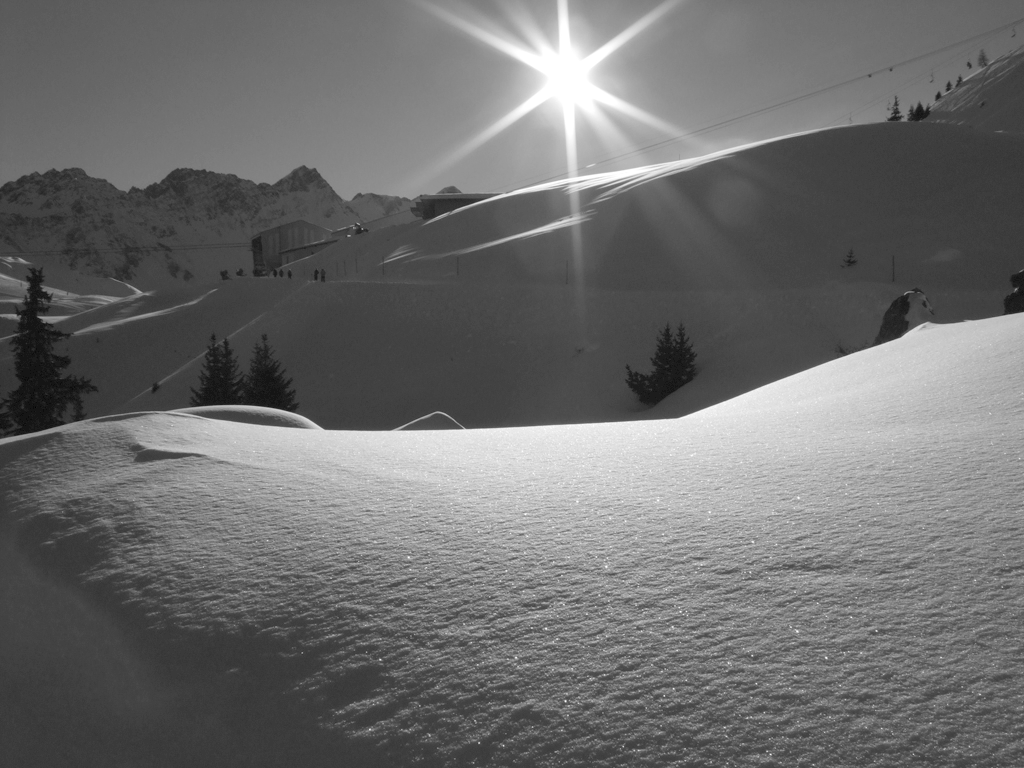
\includegraphics[width=0.8\textwidth]{pics/grau}
    \end{center}
    \caption{Ein Bild mit etwas mehr Informationen (und etwas mehr Speicherplatzbedarf:
551kb)}
  \end{figure}
\end{frame}
%
\begin{frame}{}
  \begin{figure}
    \begin{center}  
      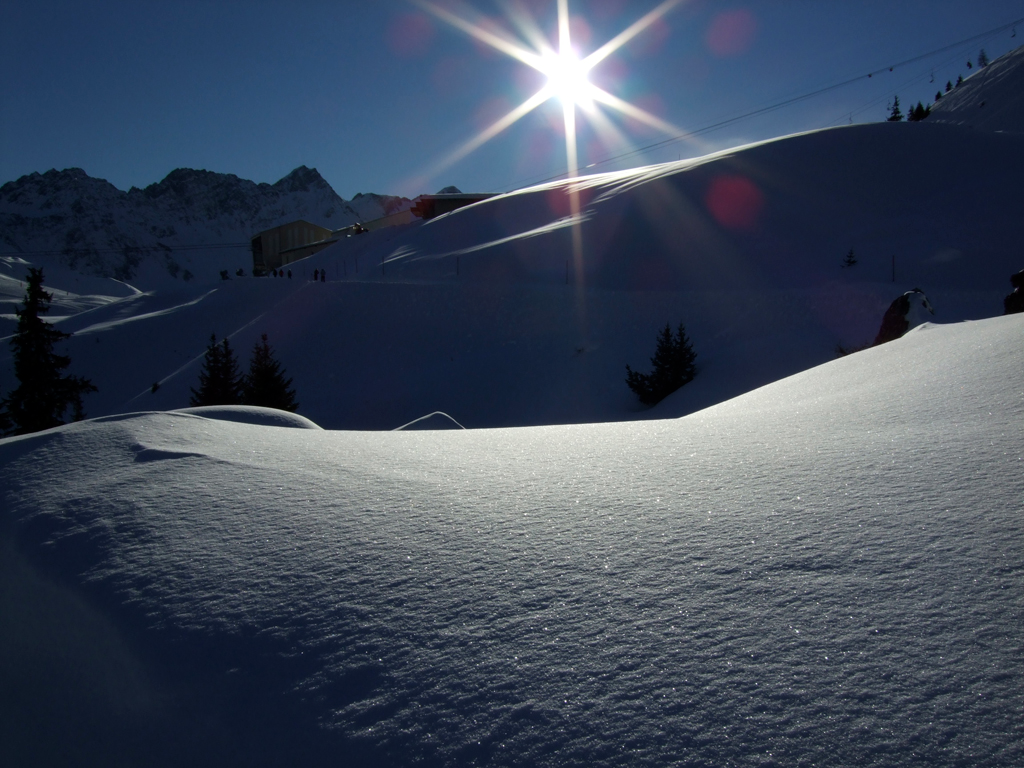
\includegraphics[width=0.8\textwidth]{pics/farbe}
    \end{center}
    \caption{Ein Bild mit vielen Informationen (und noch mehr Speicherplatzbedarf:
1,1 MB)}
  \end{figure}
\end{frame}
%
\begin{frame}
\frametitle{Je mehr, desto besser}
  Je mehr ,,an'' / ,,aus'' Informationen wir einsetzen, desto näher ist das Ergebnis an der Wirklichkeit. Entsprechend steigen aber auch die benötigte Rechenleistung und der Speicherplatzbedarf an. 
\end{frame}
%
\only<article>{
  Das sind nun relativ kleine Beispielbilder gewesen. Rohbilder moderner Kameras benötigen aktuell 25 MB pro Bild, im semiprofessionellen Bereich das Doppelte, und im Mittelformat braucht es pro Bild ca. 600MB. Deshalb rechnet man mit speziellen Algorithmen ,,nicht benötigte'' Informationen aus den Daten heraus. Auch wenn der Leistungszuwachs von Computern aussergewöhnlich ist, stehen Speicher und Rechenpower nicht unbegrenzt zur Verfügung und sollten ganz normal als Ressource wahrgenommen werden, die man nicht verschwendet. 
  }

\subsection{Die Entwicklung des Internets}
%
\begin{frame}[<+->]{\only<presentation>{Die Entwicklung des Internets}}
\framesubtitle{Meilensteine}
  \begin{itemize}
    \item ARPA
    \item E-Mail
    \item www --- ein neuer Treiber
    \item Web Apps, Cloud Services und intelligente Kühlschränke
  \end{itemize}
\end{frame}

\subsubsection*{Der Vorläufer des Internets: Das Arpanet}
%%%%
%% Bis hier bin ich mit dem Refactoring gekommen
%%%%
\only<article>{
  Das Internet ist 1969 aus einer Zusammenarbeit des US--Verteidigungsministeriums und verschiedenen Forschungseinrichtungen entstanden. Obwohl sich das Gerücht hält, dass im kalten Krieg eine Technik aufgebaut werden sollte, die im Falle eines Atomschlages die Kommunikationsinfrastruktur erhalten kann, dürfte ein ausschlaggebender Grund für die Entwicklung die bessere Ausnutzung teurer Rechenkapazitäten gewesen sein. So entstand als Vorläufer des heutigen Internets das Arpanet. So oder so --- die Idee ist genial: Man teilt Kommunikation in kleine Päckchen auf und entwickelt Protokolle, die es ermöglichen, dass sich diese Päckchen ihren Weg selbständig vom Sender zum Empfänger suchen. Dabei gibt es nicht nur eine Leitung von A nach B, sondern ein fein verzweigtes Netzwerk mit unzähligen Knoten. Wenn nun eine Leitung blockiert ist, nimmt das Päckchen einfach einen anderen Weg. Übertragen wurden damals Übrigens noch keine Webseiten mit Bildern.
  }

\subsubsection{www : am CERN wird Internet--Geschichte geschrieben}

\only<article>{Das CERN spielt eine wichtige Rolle bei der Entwicklung des Internets, wie wir es heute kennen. Die Laboratorien des CERN liegen teilweise auf Schweizer Gebiet, teilweise auf französischem. Natürlich setzt jedes Land seine eigenen Computersysteme ein, was es damals unmöglich machte, Texte online auszutauschen. Mitte der achtziger Jahre nahm sich ein britischer Physiker und Informatiker namens Tim Berners--Lee dieses Problems an und entwickelt mit seinem Kollegen Robert Cailliau ein Konzept für ein weltweites Hypertext--Projekt, das sie 1990 veröffentlichen. Das daraus entstehende Protokoll ,,http" und die Auszeichnungssprache ,,html'' sind auch heute noch die Grundlagen des \textbf{W}orld \textbf{W}ide \textbf{W}eb. Dabei geht es darum Texte Über das Netzwerk zur Verfügung stellen zu können. Die Problematik, Texte universell für verschiedenste System darstellbar zu Übertragen, wird auch heute noch deutlich, wenn man z.B. eine Webseite auf einem Smartphone öffnet, die für den Desktop optimiert ist. Inzwischen sind die Texte um Bilder ,,bereichert", Filme werden Über das Internet gestreamt und Weltkarten in 3D betrachtet.
}

\subsubsection*{Das Internet der Dinge}

\only<article>{Da man nun immer mehr Leistung in immer kleinere Chips packen kann, können kleinste Dinge Funktionen bekommen, für die man früher ganze Rechenzentren benötigte. Wecker zeigen das Wetter an, Kalender berechnen die Wegzeit automatisch in Alarme mit ein, Navigationssysteme verwenden aktuelle und zu erwartende Verkehrsdaten, um die optimale Route zu bestimmen. Für all das benötigen die Dinge eine Verbindung zum Internet. Das wirft verschiedene Probleme auf: Sicherheit und Datenschutz sind ein Thema. Aber auch technisch braucht es neue Ansätze. So muss jeder, der an ihn gerichtete Informationen bekommen will, eindeutig identifizierbar sein. Die ursprünglich für diesen Zweck gemachte Adressierung (IPv4) hat für das Internet der Dinge viel zu wenig Adressen. Eine neue Technik zur Adressierung --- IPv6 --- ist vorhanden, setzt sich aber nur langsam durch.}

\begin{frame}
  \begin{figure}
    \begin{center}  
      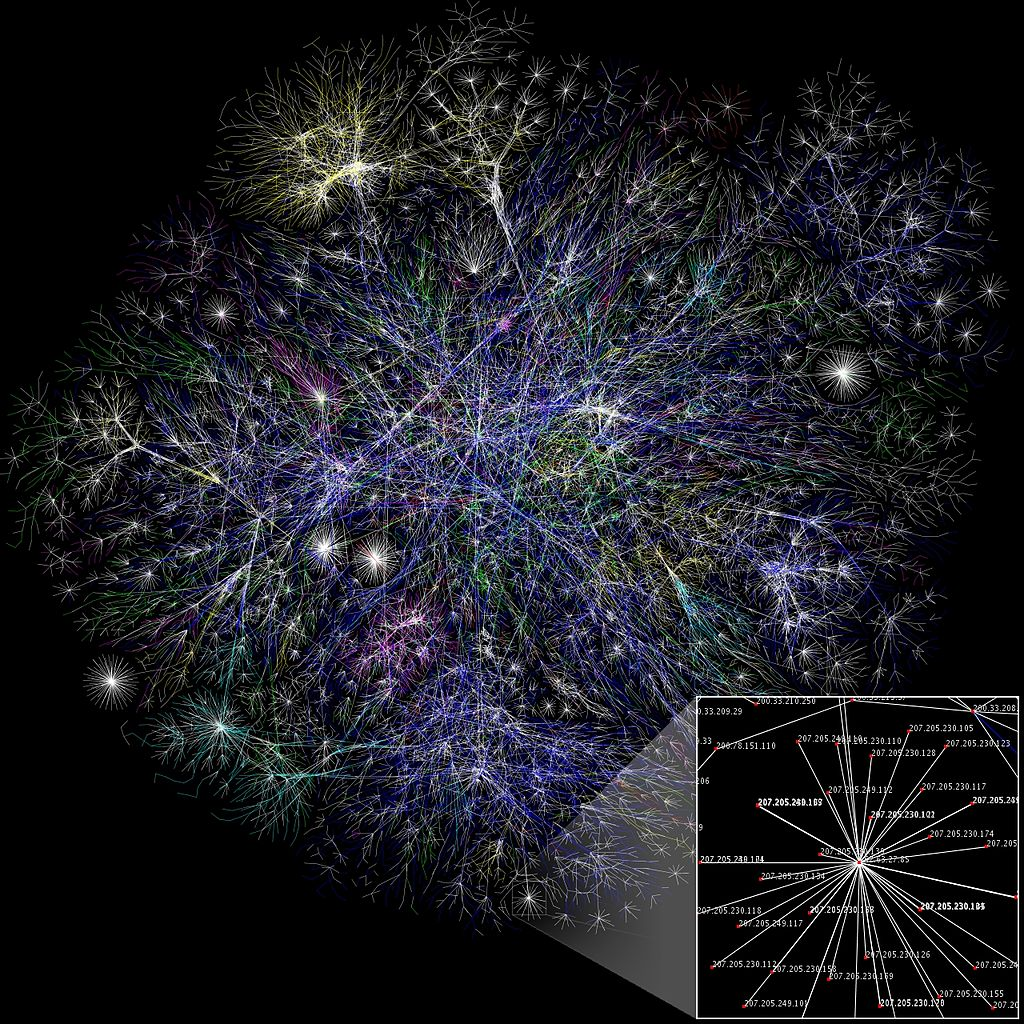
\includegraphics[width=0.6\textwidth]{pics/internet}
    \end{center}
    \caption{Das Internet heute; Quelle: Wikipedia, Urheber: The Opte Project}
  \end{figure}
\end{frame}


\subsection{Server --- was ist das eigentlich?}
\begin{frame}[<+->]{\only<presentation>{Server --- was ist das eigentlich?}}
  \framesubtitle{die Themen:}
  \begin{itemize}
    \item Hardware
    \item Virtualisierung
    \item Software
  \end{itemize}
\end{frame}
%

\subsubsection*{Hardware}
\begin{frame}{}

\begin{figure}
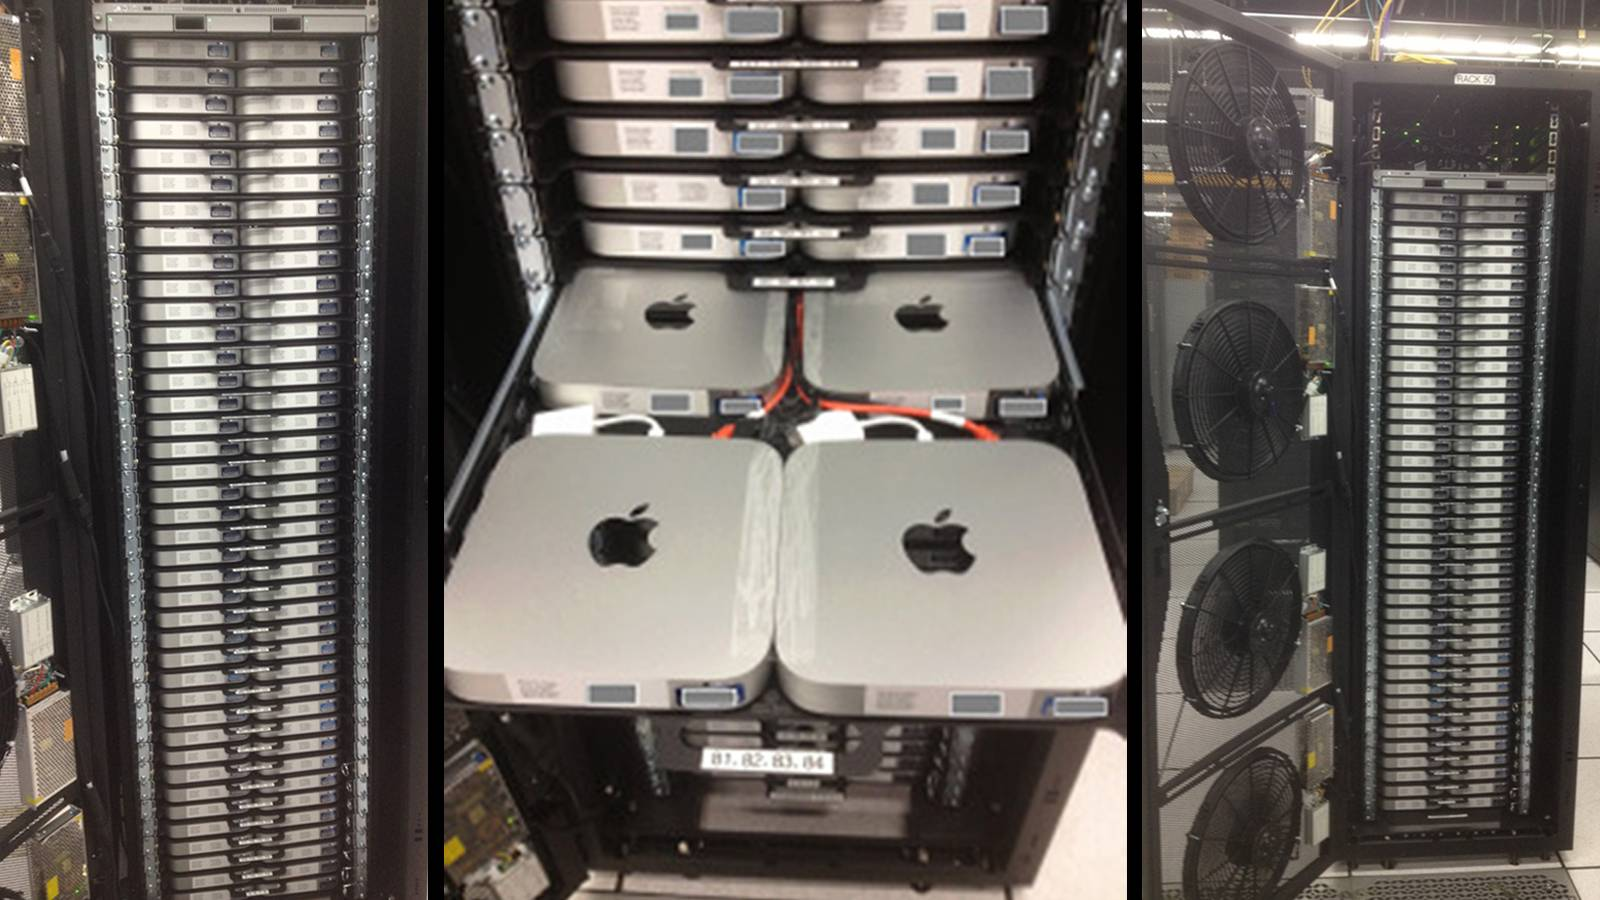
\includegraphics[width=1\textwidth]{pics/MacMiniServer}

\caption{MacMini Server; Quelle: Gizmodo India}
\end{figure}

\end{frame}
\only<article>{
  Was ist ein Server? Im Grunde genommen ist jedes Gerät, das Dienstleistungen zur Verfügung stellt, ein Server. Wenn ich von meinem lokalen PC eine Webseite bereit stelle, die jemand anderes von seinem PC aufruft, ist mein PC in dem Moment ein Server.

  Ursprünglich war Rechenleistung so teuer, dass es in einer Institution nur einen riesigen Rechner in einem gut gekühlten Keller gab. Terminals ohne eigene Rechenkapazität stellten für eine Anzahl von Nutzern eine Verbindung zu diesem Rechner her, dessen Leistung unter allen Nutzern aufgeteilt wurde. Ende der 70er Jahre wurde die Technik so billig, dass mit dem Aufkommen der Personal Computers jeder seinen eigenen Rechner auf seinem Schreibtisch hatte. 

  Im Jahr 2000 wurden für den Aufbau einer Datenbank für kurze Texte noch 40.000 DM für einen Server der Firma SUN ausgegeben. Der Vorschlag, stattdessen einen Linux--PC für 5'000 DM einzusetzen war revolutionär\ldots{} und erfolgreich. Tatsächlich waren die PCs so leistungsfähig geworden, dass es keinen Grund mehr gab, das Achtfache zu investieren. 

  Woraus besteht nun ein PC?
}

\begin{frame}{die Komponenten eines PCs}

\begin{figure}
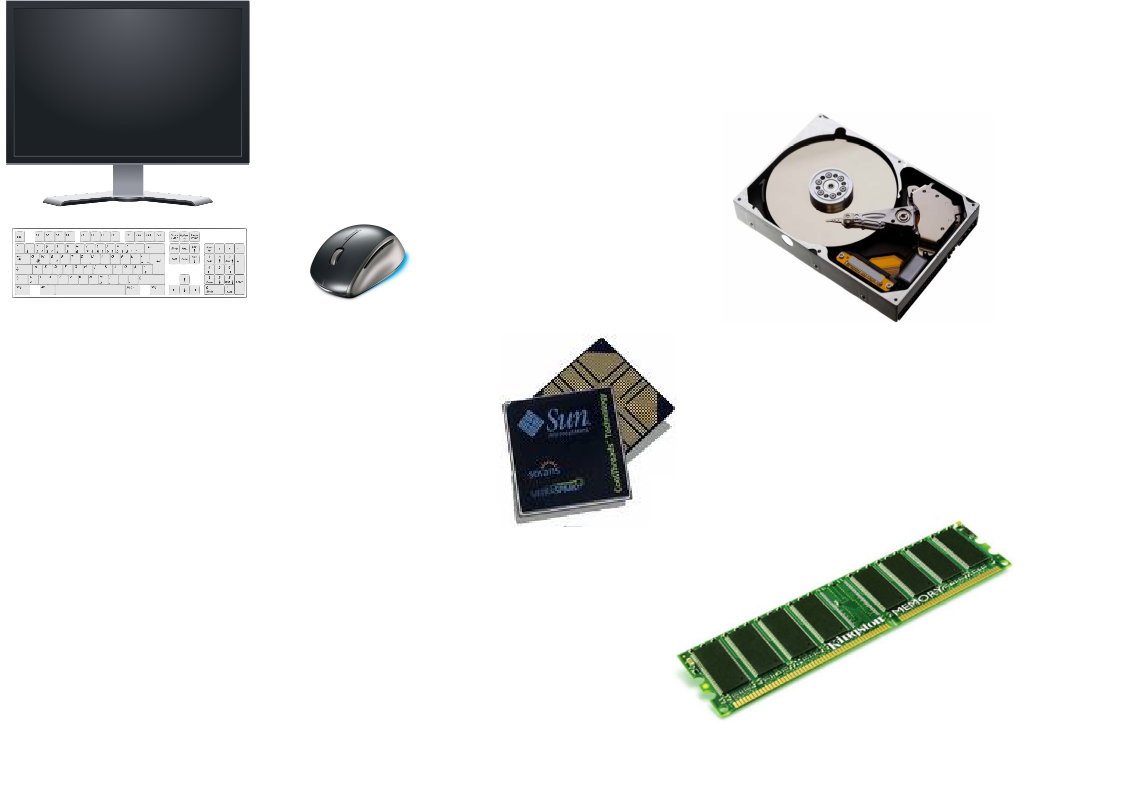
\includegraphics[width=1\textwidth]{pics/pc-komponenten}

\caption{die Komponenten eines PCs}
\end{figure}
\end{frame}

\only<article>{
  Das Herzstück des PCs ist der Prozessor --- der eigentliche Rechner. Damit Menschen mit ihm kommunizieren können, gibt es Ein-- und Ausgabesysteme. Bis in die achtziger Jahre wurden dafür z.B. Lochkarten gebraucht, heute benutzen wir im Wesentlichen Tastatur und Maus, immer öfter auch den Touchscreen. Monitore und Drucker sind Beispiele für Ausgabesysteme. 
  
  Die Daten müssen irgendwo gespeichert werden. Auch hierfür taugt die Lochkarte bzw. ganze Lochbänder, inzwischen abgelöst durch magnetische Medien, optische Datenträger und nichtflüchtige elektronische Speicher. "Nichtflüchtig'' leitet zu einem weiteren Speicher Über: Der Prozessor eines PCs ist so schnell, dass er einen besonderen, schnellen Zwischenspeicher benötigt, von dem er Daten laden und auf dem er seine Ergebnisse ablegen kann. Die Rede ist vom RAM, ein schneller elektronischer Speicher, der allerdings seine Informationen sofort verliert, wenn der Strom abgeschaltet wird.

  Auf den meisten Heim-- PCs ist heutzutage nicht mehr der Prozessor (CPU) der schnellste im Team. Den Titel hat er an den Grafikprozessor (GPU) abgegeben. Dazu muss man wissen, dass die Spieleentwicklung einer der Treiber bei der technischen Entwicklung von PCs ist. Und für Bilder gilt genauso wie für alles Digitalisierte: Je wirklichkeitsgetreuer die Darstellung sein soll, desto mehr ,,AN'' / ,,AUS" Informationen brauchen wir, und desto leistungsfähiger muss die Hardware sein. 

  Verbunden werden all die Komponenten durch das sogenannte Motherboard. Auf ihm sitzt auch ein weiterer kleiner Chip, der beim Einschalten des PCs erstmal die Komponenten sortiert und entscheidet, was gestartet werden soll. Das Problem ist nämlich, dass kein Bauteil vom anderen "weiss". Wir brauchen eine Software, die die Bauteile miteinander verknüpft, das Betriebssystem. Das Betriebssystem Übernimmt vom Chip die Hoheit Über den Computer und stellt uns unsere Arbeitsumgebung --- im Alltag also den Desktop mit Mail--Programm, Textverarbeitung usw. --- zur Verfügung.
}

\subsubsection*{Server: Software}

\only<article>{
  Das Wort Server wird synonym auch für die Software benutzt, die dafür zuständig ist, Services zu erbringen. Wenn wir von einem Webserver sprechen, kann sowohl die (virtuelle) Maschine gemeint sein, die die Webseiten ausliefert, als auch die Software --- z.B. Apache, nginx, puma etc. --- auf der Maschine, die diese Arbeit Übernimmt.
}

\begin{frame}[<+->]{Beispiele für Software-- Server}
  \begin{itemize}
    \item Webserver
    \item Mailserver
    \item Dateiserver
    \item Datenbankserver
  \end{itemize}
\end{frame}

\only<article>{
  Immer Übernimmt eine entsprechende Software die Aufgabe, Daten auszuliefern bzw. zu empfangen. Auf einem Hardwareserver können mehrere Softwareserver laufen, auch wenn es im Zuge der Virtualisierung sinnvoll erscheint, für jeden Serverzweck eine eigene virtuelle Maschine zu Verfügung zu stellen. So läuft in der ETH--Bibliothek z.B. das Bibliothekssystem auf einem vituellen Server, die Datenbank auf einem anderen.
  }

\subsection{enorme Leistungssteigerung}
\only<article>{
  Das Moorsche Gesetz besagt dass sich die Rechenleistung alle ein bis zwei Jahre verdoppelt. Inzwischen haben wir mehr Leistung in einem Mobiltelefon, als noch vor zehn Jahren auf dem Desktop.

  Wie konnten diese bemerkenswerten Leistungssteigerungen erzielt werden? Stark vereinfacht (und anders als beispielsweise in der Chemie) mit der Formel ,,viel hilft viel''.

  Vor noch gar nicht so langer Zeit wurden Daten auf einer sogenannten Festplatte gespeichert. In einem luftdichten Gehäuse wurde eine beschichtete Platte zum Rotieren gebracht und mit einem Lese--/Schreibkopf die Daten darauf magnetisch abgelegt bzw. ausgelesen. Um die Geschwindigkeit zu erhöhen lies man zum einen die Platten immer schneller rotieren, zum anderen erhöhte man die Dichte der magnetisierbaren Partikel auf der Platte, so dass bei gleicher Rotationsgeschwindigkeit mehr Informationen am Kopf vorbei kamen.

  Was macht man, wenn die Platte voll ist? Man kauft eine zweite. 

  Findige Köpfe kamen auf die Idee, die zweite Platte in das selbe Gehäuse einzubauen. Inzwischen besteht eine Festplatte aus einem Plattenstapel, in dessen Zwischenräumen die Köpfe kammartig greifen und die Informationen schreiben bzw. lesen. Durch die gleichzeitigen Schreib-- und Lesevorgänge konnten neben dem erhöhten Speicherplatz auch die Geschwindigkeit weiter gesteigert werden.

  Ein ähnliches Prinzip fuktioniert auch bei Prozessoren: Statt einem benutzt man mehrere gleichzeitig, und da man dank des Fortschritts in der Halbleitertechnologie immer mehr Transistoren auf immer kleinerem Raum unterbringt, kann man in einem Prozessor mehrere Kerne realisieren, so dass mehr Operationen gleichzeitig ausgeführt werden können.
}

\subsection{Virtualisierung}

\begin{frame}{\only<presentation>{Virtualisierung}}

\begin{figure}
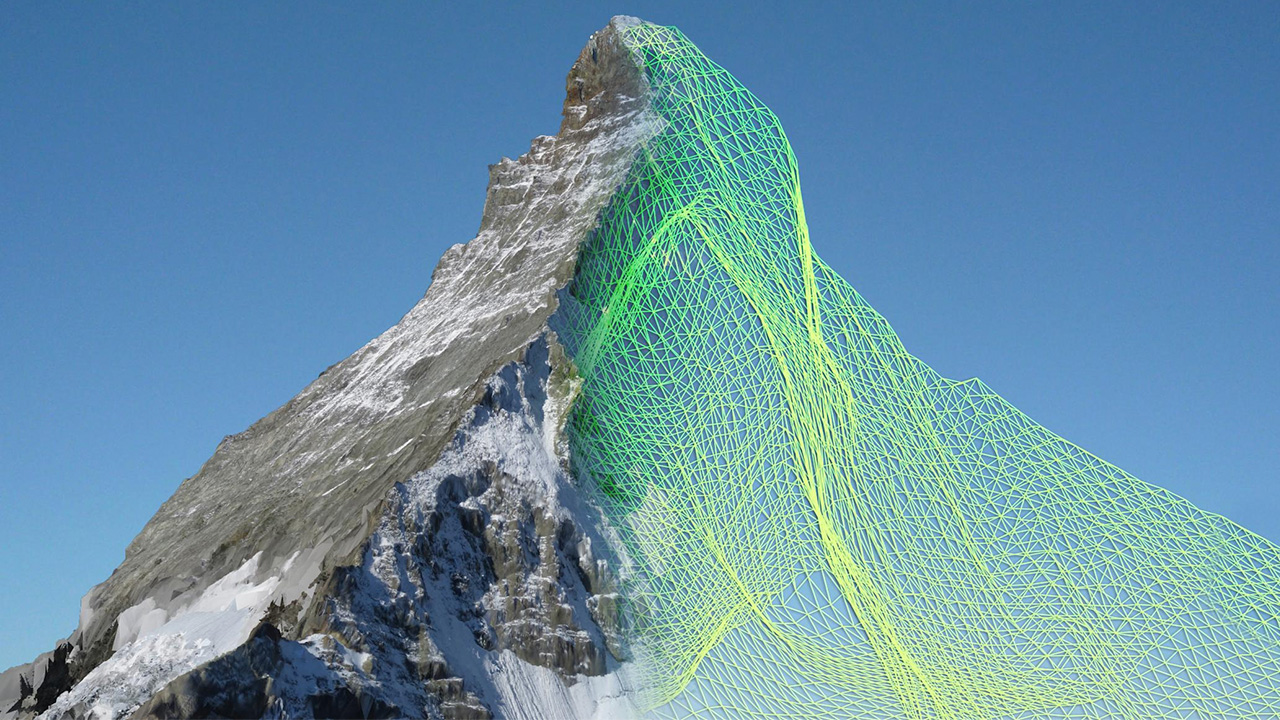
\includegraphics[width=1\textwidth]{pics/Matterhorn}

\caption{Photomontage: Jamani Caillet / © EPFL\newline           \hspace{\linewidth}http://actu.epfl.ch/news/the-matterhorn-like-you-ve-never-seen-it/}
\end{figure}
\end{frame}
\only<article>{
  Hardware ist so billig --- warum sollte man einen PC virtualisieren wollen? 
  
  Seit Microsoft mit seinen Produkten den PC--Markt beherrscht, stellt sich für Nicht--Windows--Nutzer ein Problem: Durch die enorme Verbreitung von Winows im PC--Markt gibt es viel Software, die ausschliesslich für Windows geschrieben wird. Was macht man nun als Benutzer eines anderen Betriebssystems, wenn man diese Software nutzen möchte? 
  
  Da seit einiger Zeit ein PC genug Leistung für zwei hat, sind kluge Köpfe auf die Idee gekommen, einen PC innerhalb eines PCs zu simulieren.

  Der Clou ist, dass man alle Komponenten eines PCs entweder teilen oder komplett simulieren kann. Wenn ein PC beispielsweise 8GB RAM hat, dann kann man 4GB davon für einen virtuellen PC benutzen. Unserem PC, unserem Betriebssystem stehen dann nur noch 4GB zur Verfügung, die Übrigen 4GB ,,gehören'' der virtuellen Maschine.

  Man ruft also auf seinem echten PC ein Programm auf, das per Software nun alle Komponenten eines PCs noch einmal simuliert und diesen virtuellen PC startet. Eine Festplatte in diesem ,,PC" ist dabei nur eine grosse Datei auf unserer echten Festplatte. Und in diesem virtuellen PC lässt sich dann ein eigenes Betriebssystem installieren. Auf diesem Weg hat man nun auf einem PC gleichzeitig Windows und Linux zur Verfügung.

  Da die Leistungsfähigkeit der Hardware inzwischen so stark gestiegen ist, kann man auf einem Computer gleichzeitig mehrere virtuelle PCs starten.
}

\begin{frame}[<+->]{Vorteile der Virtualisierung}
  \begin{itemize}
    \item Da virtuelle Computer nur Dateien auf einer Festplatte sind, kann man sie komplett in einem Backup sichern und quasi auf Knopfdruck wieder herstellen.
    \item Wenn man für einen Computer kurzfristig mehr Leistung braucht, kann man einem virtuellen Computer einfach per Software mehr RAM oder weitere CPUs zur Verfügung stellen. Das geht teilweise unterbruchsfrei.
    \item Computer sind selten ausgelastet. Wenn man seinen Bedarf auf virtuelle Maschinen verteilt, ist die Auslastung der echten Systeme besser.
  \end{itemize}
\end{frame}

